\chapter{Úvod}
  Odtlačky prstov sú komplikovanou spleťou cestičiek, ktoré sa navzájom krížia, spájajú a ukončujú, vytvárajú slepé uličky alebo diaľničné uzly.
  Kombinácie týchto vlastností cestičiek vytvárajú unikátny podpis ich vlastníka. Tieto cestičky, nazývané papilárne línie, sú pozorovateľné
  voľným okom a sú kategorizovateľné, čo znamená, že ich unikátnosť je možné využívať v rôznych smeroch bezpečnosti. Spočiatku sa odtlačky prstov
  využívali v kriminalistike, kde rýchlo nabrali na popularite a ich využitie bolo čím ďalej, tým viac rozšírené. S~príchodom výpočtových systémov
  sa ich analýza začala automatizovať, čo znamenalo digitalizáciu záznamov, prispôsobovanie rôznych matematických konštrukcií pre zjednodušenie ich
  analýzy počítačmi a celkové rozšírenie znalostí o odtlačkoch prstov. 
  
  Koncom minulého storočia sa navrhlo množstvo rôznych prístupov k spracovaniu odtlačkov prstov, ktoré boli časom vylepšené, prípadne integrované
  medzi sebou. Základné princípy automatizovanej analýzy sú však zväčša nemenné. Väčšina metód sa spolieha na viackrokové predspracovanie
  vstupnej snímky a následnú analýzu upravenej snímky. Predstavením základných pojmov skúmania odtlačkov prstov a takýmto spôsobom ich analýzy
  sa zaoberá kapitola \ref{kap:odtlacok}.

  Digitalizácia záznamov odtlačkov prstov v Spojených štátoch amerických predstavovala veľkú výzvu pre dátové skládky tamojších kriminalistických orgánov, pretože 
  metódy kompresie snímok neboli v tej dobe prispôsobené zachovávaniu detailov potrebných pre bezproblémovú analýzu odtlačkov prstov 
  po kompresii. Ako riešenie Americký Federálny úrad pre vyšetrovanie (FBI) implementovalo novú metódu kompresie snímok založenú na diskrétnej vlnkovej transformácii
  vo formáte vlnkového skalárneho kvantovania (WSQ). Súborom WSQ a~spôsobu kompresie v tomto formáte sa venujem v kapitole \ref{kap:wsq}.

  Vzhľadom na množstvo rôznych úkonov spojených s analýzou odtlačkov prstov je pri študovaní týchto úkonov nápomocné mať vizuálne pomôcky
  pre demonštráciu procesov s nimi spojených. Obrázky a náčrty v študijných materiáloch sú samozrejme veľkou pomôckou, avšak nemusia vždy
  poskytnúť tie informácie, ktoré študent potrebuje. Výstup tejto práce má za cieľ poskytnúť aplikáciu, ktorá je schopná reprodukovať
  niektoré najbežnejšie úkony predspracovania a analýzy snímok odtlačkov prstov tak, aby užívateľovi demonštrovali význam jednotlivých úkonov
  interaktívnym spôsobom na snímkach dodaných samotným užívateľom. Návrh aplikácie je popísaný v kapitole \ref{kap:navrh_appky}.
  
  % //TODO: ak bude dalsia kapitola, tak v kratkosti este popisat aj tu

\chapter{Odtlačok prsta} \label{kap:odtlacok}
  Každý človek na svete je unikátne identifikovateľný podľa odtlačkov prsta. Ako prvý publikoval význam odtlačkov prstov zanechaných na miestach činu
  pre identifikáciu jednotlivcov Henry Faulds. V roku 1880 publikoval článok v žurnále \emph{Nature} informujúci výskumníkov o jeho zisteniach o unikátnosti
  a permanencii papilárnych línii. V danom článku opísal dva konkrétne prípady, kde boli využité odtlačky prstov na individualizáciu osôb a navrhol
  používanie takéhoto spôsobu identifikácie na miestach činu. V roku 1892 sir Francis Galton napísal prvú knihu o odtlačkoch
  prstov \emph{Finger Prints}, v ktorej definoval a pomenoval špecifické markanty odtlačkov prstov \cite{FingerprintSrcBook}.
  V tejto kapitole bude poskytnutý prehľad o biológii kože, klasifikácii odtlačkov prstov a o spôsoboch automatizovanej analýzy týchto odtlačkov.
  
  %Toto je vďaka vývojovým procesom,
  %ktoré sa začnú v ľudskom embryu približne jedenásť týždňov od oplodnenia, keď sa začnú na prstoch embrya vytvárať papilárne línie.
  %Tieto procesy, podobne ako napríklad procesy, ktoré zabezbečujú vývoj žíl a ciev v ľudskom tele, sú pre každého jedinca neidentické.
  %Papilárne línie sú tvorené vonkajšou vrstvou kože, epidermou, na prstoch rúk a nôh. Po úplnom vyvinutí papilárnych línií sa po celý život jedinca
  %bez vonkajšieho zásahu nijak zásadne nezmenia. Odtlačok zanechaný na povrchoch materiálov osobou, ktorá sa ho dotkne je obecne nazývaný odtlačkom prstu.
  
  \section{Koža a jej štruktúra}
  Ľudská koža je orgán obklopujúci ľudské telo plniaci mnoho účelov. Troma hlavnými účelmi kože sú ochrana pred vonkajšími vplyvmi, regulácia
  telesných charakteristík (napr. telesná teplota) a zmyslové vnímanie okolitého sveta.
  Koža sa skladá z troch hlavných vrstiev: pokožka (epidermis), zamša (dermis) a podkožné väzivo (hypodermis). Tieto vrstvy sa ešte môžu ďalej deliť
  na ďalšie podvrstvy podľa účelu alebo biologického zloženia danej podvrstvy.

  \subsection{Pokožka}
  Pokožka je najvonkajšou časťou kože, ktorá je vrstvená periodicky sa regenerujúcim epitelovým tkanivom. Toto tkanivo má rôzne funkcie v rôznych
  častiach ľudského tela, pričom v prípade pokožky plní účel prevencie straty tekutín a vody, prieniku látok z vonkajšieho prostredia do tela, ale aj
  mechanickej ochrany. Táto vrstva epitelového tkaniva je avaskulárna, čo znamená, že sa v nej nenachádzajú cievy, a teda pokožkové bunky prijímajú živiny
  najmä zo spojového tkaniva zamše.
  
  Pokožka nie je homogénna z hľadiska typov buniek v nej obsiahnutých, avšak značná väčšina (90 - 95\% buniek) sú keratinocyty. V priebehu 
  ich životného cyklu keratinocyty prejdú tzv. diferenciáciou, čo vo vývinovej biológií znamená, že bunka jedného typu (obvykle kmeňová a  málo špecializovaná)
  prejde zmenami, vďaka ktorým sa vyvinie do bunky iného typu (úzko špecializovanej bunky) \cite{slack2012biology}. Pokožku je možné deliť na ďalšie
  vrstvy znázornené na \ref{obr:pokozka_vrstvy}, ktoré sú úzko spojené so štádiami diferenciácie keratinocytov. Keratinocyty sa v pokožke vyvíjajú
  z kmeňových buniek v najhlbšej vrstve stratum basale a počas diferenciácie migrujú k povrchu pokožky tiež nazývanou stratum corneum. V tejto vrstve sa 
  prevažne nachádzajú tzv. korneocyty, čo sú keratinocyty na konci procesu diferenciácie. Tieto bunky sú zrohovatenými keratinocytmi bez bunečného jadra
  a cytoplazmatiských organel \cite{koster2009epidermis}. Korneocyty sa následne odlupujú od pokožky pri procese deskvamácie. Celý proces migrácie
  keratinocytov po opustení stratum basale až po stratum corneum obyčajne trvá aspoň 14 dní, pričom deskvamácia trvá prinajmenšom ďalších 14 dní.

  \begin{figure}[h]
    \centering
    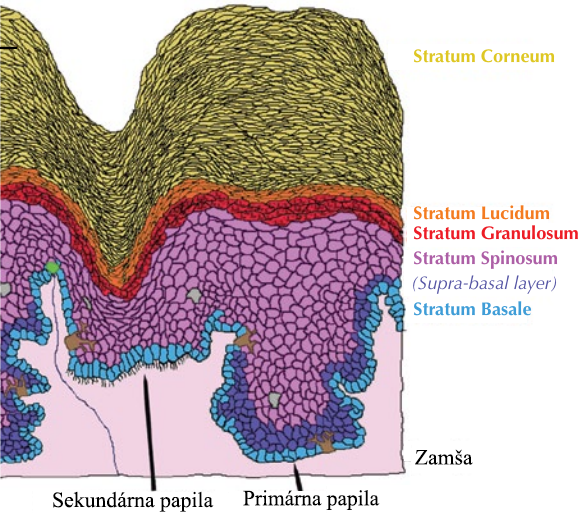
\includegraphics[width=0.6\linewidth]{obrazky-figures/pokozka_vrstvy.png} % TODO: mozno nahradit za obrazok z public domain?
    \caption{Vrstvy pokožky. Prevzaté z \cite{FingerprintSrcBook}.}
    \label{obr:pokozka_vrstvy}
  \end{figure}

  \subsection{Zamša}
  Pod pokožkou sa nachádza zamša, ktorá poskytuje koži jej elasticitu a pevnosť v ťahu (pevnosť materiálu pri naťahovaní). Je to spojivové tkanivo,
  a teda na rozdiel od pokožky je táto vrstva kože omnoho menej bunečná. Skladá sa hlavne z vláknitej a amorfnej medzibunkovej hmoty, pomocou ktorej dodáva
  živiny bunkám v pokožke. Hlavnými typmi vláknitého spojivového tkaniva v tejto vrstve sú kolagén a elastické spojivové väzivo, z čoho práve kolagén je
  najviac zastúpený v zamši so zastúpením približne 75\% suchej váhy kože. Štrukturálne je zamša rozdelená na dve vrstvy - papilárna vrstva (stratum papilaris)
  a vláknitá vrstva (stratum reticularis).

  \textbf{Papilárna vrstva} je primárne zložená z malých zhlukov kolagénových fibríl malého priemeru a oxytalánových elastických vlákien.
  Plní úlohu spoju zamše s pokožkou. Ako je znázornené na obrázku \ref{obr:zamsa_a_papily/zamsa}, papilárna vrstva zamše má tvar údolí a vrchov
  nielen vo volárnych (vnútorná strana ruky) a stupajových častiach kože, kde je takáto štruktúra tvorená aj na pokožke (tzv. papilárne valy), ale aj na miestach,
  kde je pokožka hladká. Vďaka tvaru papilárnej vrstvy sa značne zvyšuje rozloha spoja medzi zamšou a pokožkou, čím sa, mimo iného, zosilňuje tento spoj.
  Týmito papilárnymi útvarmi sa prelínajú drobné krvné cievy - vlásočnice, ktoré zabezpečujú prívod živín a pomocou nich sa vykonáva aj regulácia telesnej
  teploty ich zúžením alebo rozšírením podľa potreby. V zamšových papilách sa nachádzajú aj nervové zakončenia vnímajúce externé stimuly ako sú napr. teplo a tlak. 

  \textbf{Vláknitá vrstva} je oproti papilárnej zložená z kolagénových fibríl väčšieho priemeru, ktoré sa zamotávajú do veľkých zväzkov vlákien,
  okolo ktorých sa obmotávajú ďalšie elastické vlákna, čím sa značne zosilňuje ich mechanická odolnosť a pružnosť. Obecne sa tieto štruktúry zväzkov zväčšujú
  s narastajúcou hĺbkou smerom k podkožnému väzivu. V tejto vrstve sa nachádzajú vetvy autonómneho nervového systému, ktorým sa riadia telesné úkony ako potenie
  ale aj krvný tok.

  Vďaka značnému prekrveniu tejto časti kože sa tu vyskytujú mnohé iné štruktúry, jednou z ktorých sú potné žľazy. Existuje viacero typov ľudských
  potných žliaz, ako napr. apokrinné, ekrinné a apoekrinné. Ďalšie delenie, hlavne apokrinných, potných žliaz je možné podľa špecializácie daných žliaz.
  Výskyt apokrinných potných žliaz je obmedzený iba na niekoľko oblastí ľudského tela. Na druhej strane sa ekrinné žľazy vyskytujú na väčšine plochy
  ľudského tela, čím sú aj najpočetnejšie pri počte dvoch až piatich miliónoch žliaz. Ich účelom je primárne regulácia telesnej teploty a udržiavanie homeostázy.
  Oblasťami najhustejšieho zastúpenia týchto žliaz sú dlane a chodidlá, kde sa ich počet pohybuje okolo 2500 - 3000 na 2.5cm\textsuperscript{2}.
  Ekrinné žľazy sú klasifikované ako jednoduché rúrkovité žľazy, ktorých vývody vyúsťujú do voľným okom neviditeľných potných pórov. Tieto póry majú
  na papilárnych valoch veľkosť približne 30\textmugreek{}m. V oblastiach papilárnych valov póry sledujú priebeh papilárnych línií a objavujú sa na ich vrcholoch,
  ako je vidno na \ref{obr:zamsa_a_papily/papily_prierez}.
  
  \begin{figure*}[h]\centering
    \centering
    \begin{subfigure}[b]{0.49\linewidth}
      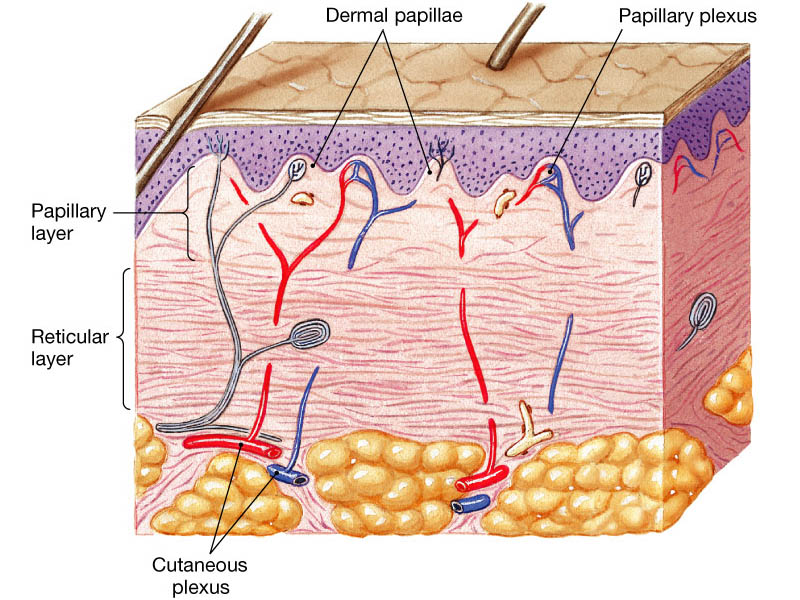
\includegraphics[width=\linewidth]{obrazky-figures/zamsa.jpg}
      \caption{Vrstvy a biologické štruktúry zamše. Prevzaté z \cite{droual_dermis}.}
      \label{obr:zamsa_a_papily/zamsa}
    \end{subfigure}
    \hfill
    \begin{subfigure}[b]{0.49\linewidth}
      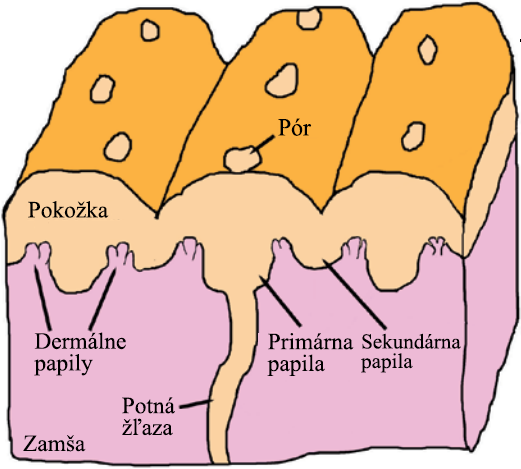
\includegraphics[width=\linewidth]{obrazky-figures/papily_prierez.png}
      \caption{Primárne, sekundárne a zamšové papily. Prevzaté z \cite{FingerprintSrcBook}.}
      \label{obr:zamsa_a_papily/papily_prierez}
    \end{subfigure}
    \caption{}
    \label{obr:zamsa_a_papily}
  \end{figure*}
  
  \subsection{Podkožné väzivo}
  Pod zamšou sa nachádza podkožné väzivo zložené prevažne z tukového tkaniva, vďaka čomu nadobúda tepelnoizolačné a ochranné vlastnosti a tiež zabezpečuje
  uskladňovanie záložnej energie. Vďaka tejto vrstve má koža schopnosť sa relatívne voľne pohybovať nad hlbšími štruktúrami tela dodávajúc koži flexibilitu.
  Často do tejto vrstvy zasahujú apokrinné a ekrinné potné žľazy a vlasové vačky s korienkami ochlpenia.

  \subsection{Papilárne línie}
  Pokožka v oblastiach dlaní a chodidiel nemá hladký povrch ako na zvyšku tela. Tieto oblasti pokožky majú valový priebeh a tvoria periodické vrcholy
  a údolia pozdĺž celej dlane a chodidla - papilárne línie. Ich vlnovitý tvar dodáva pokožke pružnosť a umožňuje pevnejšie uchopenie rôznych povrchov
  \cite{FingerprintSrcBook}. Pri pohľade na prierez kože na \ref{obr:zamsa_a_papily/papily_prierez} je možné pozorovať prepojenie zamše s papilárnou pokožkou.
  Papilárne línie pokožky vytvárajú primárne a sekundárne výbežky zasahujúce do zamše, zvyšujúc silu spoja týchto dvoch vrstiev kože. Cez primárne výbežky
  vedú vývody ekrinných potných žliaz vyúsťujúce do pórov na vrcholoch papilárnych valov. Papilárne línie, potné žľazy
  a iné štruktúry na povrchu kože sa v následku dotyku nejakého povrchu na ňom odtlačia a zanechajú po sebe \uv{mapu}, 
  ktorej sa všeobecne hovorí odtlačok prsta.

  Táto sekcia čerpala z \cite{freinkel2001skin} ak nie je uvedené inak.

  \section{Zaznamenávanie odtlačkov prsta}
  Od počiatkov identifikácie na základe papilárnych línií sa vyvinulo mnoho spôsobov zaznamenávania ich odtlačkov od prenášania odtlačku na papier
  za pomoci média ako atrament a následné skenovanie do digitálnej formy (tzv. off-line snímanie) cez optické snímanie až po termálne snímače
  (tzv. live-scan snímanie). Samotné snímanie je možné zobecniť na niekoľko krokov: senzor sníma analógové informácie o štruktúre papilárnych línií,
  ktoré sú následne konvertované do digitálnej podoby analógovo-digitálnym prevodníkom a následne sú nasnímané dáta prenesené cez komunikačné rozhranie
  na ďalšie spracovanie alebo uloženie. Nie vždy je však žiaduce snímané dáta prenášať na iný systém. V takýchto prípadoch sa využívajú čipové systémy,
  kde sa integruje snímanie a spracovanie na jednom čipe.
  V tejto sekcii sú v krátkosti uvedené niektoré metódy snímania.

  \subsection{Optické snímače}
  Jedná sa o relatívne jednoduchý princíp snímania svetla odrazeného papilárnymi valmi. Najstaršou variantou optických snímačov je technológia \emph{FTIR}
  (Frustrated Total Internal Reflection), kde sa špička prsta položí na základňu optického hranola, pričom svetelný zdroj (obyčajne svetelná dióda) osvecuje
  papilárne valy, z čoho je pomocou zrkadlenia cez optický hranol vytvorená snímka za pomoci CCD alebo CMOS optického senzoru. Fungovanie takéhoto snímača
  je naznačené na \ref{obr:ftir_snimac}. Použité osvetlenie by malo byť ploché, rozptýlené a nie priame, čím sa zabezpečí rovnomernejšie rozloženie svetla
  cez priložený prst. Vrcholy papilárnych línií, ktoré sú v kontakte s optickým hranolom, pohltia alebo rozptýlia značnú časť vyžarovaného svetla. Údolia,
  ktoré naopak nie sú v kontakte s hranolom, neovplyvňujú svetelné žiarenie, čím umožňujú svetlu odrážať sa priamo smerom k obrazovému senzoru. Vďaka týmto
  rozdielom svetelného rozptylu sa na snímači prejavia vrcholy ako tmavé a údolia ako svetlé body na snímke. Pre koncentráciu svetla na senzor sa využíva
  optická šošovka. Existuje viacero variácií snímania založených na princípe FTIR, ktoré boli vyvinuté s účelom zmenšiť prevedenie takýchto snímačov
  pre jednoduchšiu integráciu do systémov menších rozmerov.

  \begin{figure}[h]
    \centering
    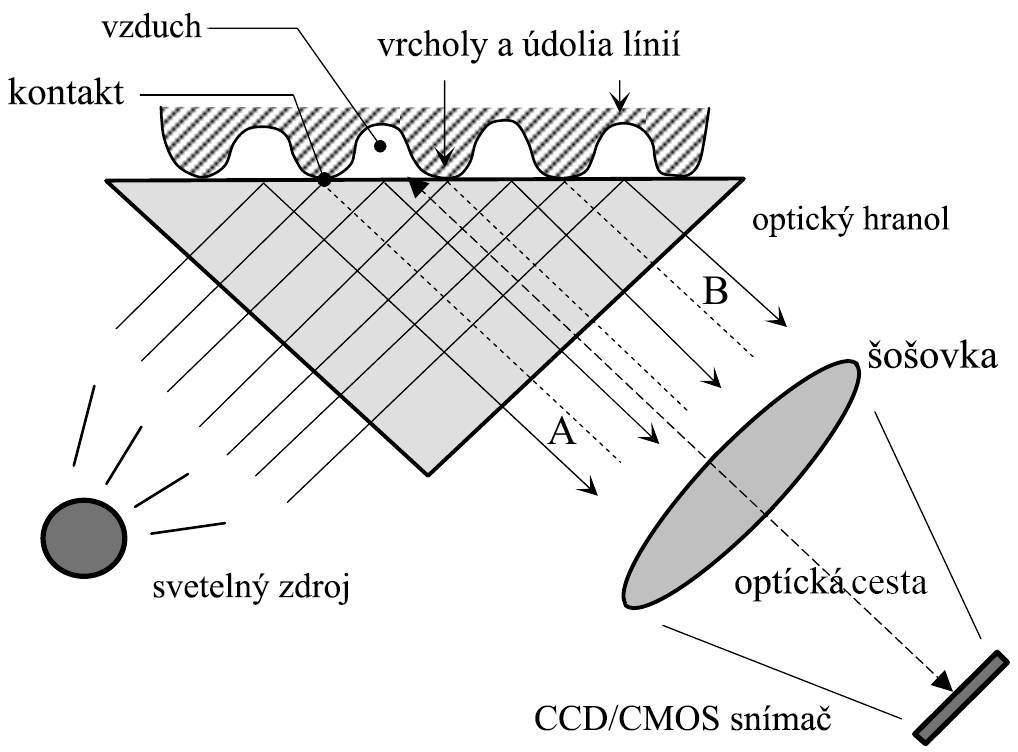
\includegraphics[width=0.6\linewidth]{obrazky-figures/ftir_snimac.png}
    \caption{Diagram znázorňujúci fungovanie FTIR snímača.}
    \label{obr:ftir_snimac}
  \end{figure}

  \subsection{Polovodičové snímače}
  Najrozšírenejším typom polovodičových snímačov sú kapacitné snímače. K rozšíreniu tohto druhu snímania prispelo rozšírenie kapacitných snímačov odtlačkov
  do väčšiny moderných smartfónov \cite{smartphone_sensors}. Kapacitné snímače odtlačkov sú založené na princípe kondenzátorov a ich schopnosti udržiavať
  elektrický náboj. Kapacitný snímač sa obecne skladá z dvoch vrstiev - izolačnej a vodivej. Izolačná vrstva sa nachádza na vonkajšej strane
  snímača, na ktorú sa položí snímaný prst. Na opačnú (vnútornú) stranu izolačnej vrstvy je naparená matica vodivých plôšok \cite{Drahansky}. Hustota týchto
  vodivých častíc musí byť vyššia, než hustota papilárnych línií kvôli zvýšeniu vzorkovacej presnosti. Pri položení prsta na snímač sa vďaka vodivosti
  pokožky a ľudského tela vytvoria malé kondenzátory tvorené prstom, izolačnou vrstvou snímača a snímacích plôšok. V týchto kondenzátoroch sa týmto vytvorí
  merateľný elektrický náboj veľkosťou závislý od vzdialenosti pokožky od náprotivných snímacích plôšok. Po interpretácií detegovaných nábojov maticou
  snímačov je možné vytvoriť snímku odtlačku prsta.
  
  \begin{figure}[h]
    \centering
    
\includegraphics[width=0.6\linewidth]{obrazky-figures/placeholder.pdf}
    \caption{Kapacitný snímač a jeho hlavné komponenty.}
    \label{obr:kapac_snimac}
  \end{figure}

  Medzi polovodičové snímače sa zaraďujú aj iné druhy, než kapacitné. Môže sa jednať napríklad o tepelné snímače, ktoré využívajú termoelektrické bunky
  registrujúce tepelné žiarenie papilárnych línií alebo tlakové snímače, ktoré využívajú piezoelektrický jav pre generovanie elektrického náboja
  pozdĺž papilárnych línií.

  \subsection{Ultrazvukové snímače}
  Takýto snímač pracuje na princípe vysielania ultrazvukového signálu a zaznamenávaní odrazu tohto signálu od objektov. Objektmi odrazené zvukové vlny
  majú rôzne vlastnosti v závislosti od materiálu a vzdialenosti daného objektu. Analýzou odrazeného signálu je možné vyčítať informácie o snímanom objekte,
  a to nie len v spojitosti s povrchom objektu, ale vďaka penetračným vlastnostiam zvukových vĺn aj o obsahu objektu. Týmto sa umožňuje jednoduchá detekcia
  falošných odtlačkov prstov. Pôvodne boli takéto snímače značne mechanické zariadenia s rotujúcimi ultrazvukovými vysielačmi a prijímačmi \cite{Drahansky},
  čím sa činili píliš nemotornými a drahými pre komerčné využitie. Časom sa výskum zameral na mikro-elektro-mechanické alternatívy ako
  CMUT (angl. capacitive micromachined ultrasonic transducer) \cite{savoia2010cmut} alebo PMUT (angl. piezoelectric-MUT) \cite{tang2015pmut}. Tieto technológie
  konvertujú pomocou kondenzátorov alebo piezoelektrikov striedavé napätie na zvukové vlny, čím slúžia ako ultrazvukové vysielače.

  \subsection{Zaznamenanie na fyzické médium}
  Najstarším a stále používaným spôsobom zaznamenávania odtlačkov prstov v kriminalistike je odtlačenie na fyzické médium ako je papier (daktyloskopické karty)
  pomocou špeciálneho atramentu. Takýto atrament je vyrábaný špecificky pre kriminalistické účely a má vhodné vlastnosti hustoty a rýchlosti sušenia pre tieto
  účely. Väčšina bežných atramentov je totiž príliš riedka alebo schne príliš pomaly, kvôli čomu sa atrament môže roztiecť a tým znehodnotiť záznam.
  V kriminalistike sa často zaznamenávajú nielen odtlačky prstov, ale celá dlaň, prípadne chodidlo - teda miesta pokožky, kde sa nachádzajú papilárne valy.

  Samotné zaznamenávanie odtlačkov prebieha prvotným nanesením tenkej vrstvy atramentu na oblasť pokožky, z ktorej sa odoberá vzorka. Nanášanie atramentu môže
  prebiehať rôzne - buď pomocou rolovania vzorkovanej časti pokožky po nanášacom pláte, ktorý je pokrytý vrstvou atramentu, alebo priamym nanesením atramentu
  nanášacím valcom. Po aplikácií atramentu sa na daktyloskopickú kartu nanesie rolovaný odtlačok. Pri odtlačkoch prstov to znamená, že sa prst priloží
  na kartu v naklonenej polohe a prst sa roluje od jednej hrany nechta po druhú. Rolované odtlačky zaznamenávajú najväčšiu (ak nie celú) plochu pokožky
  s papilárnymi valmi, čím obsahujú veľké množstvo informácií o papilárnych líniách. Na obrázku \ref{obr:druhy_odtlackov} je možné vidieť rozdiel v zaznamenanej
  ploche medzi rolovaným a obyčajným pichaným odtlačkom. Koncom dvadsiateho storočia sa z dôvodu veľkého množstva fyzických záznamov odtlačkov vo forme
  daktyloskopických kariet začali tieto záznamy digitalizovať skenovaním. Rozšírené digitálne formáty a ich vývin sú popísané v kapitole \ref{kap:wsq}.

  \begin{figure*}[h]\centering
    \centering
    \begin{subfigure}[b]{0.32\linewidth}
      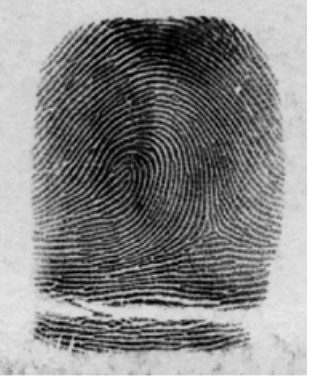
\includegraphics[width=\linewidth]{obrazky-figures/rolovany_odtlacok-Drahansky.png}
      \caption{rolovaný}
      \label{obr:rolovany_odtlacok}
    \end{subfigure}
    \hfill
    \begin{subfigure}[b]{0.32\linewidth}
      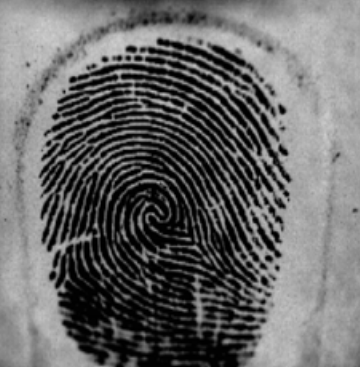
\includegraphics[width=\linewidth]{obrazky-figures/pichany_odtlacok-Drahansky.png}
      \caption{pichaný}
      \label{obr:pichany_odtlacok}
    \end{subfigure}
    \hfill
    \begin{subfigure}[b]{0.32\linewidth}
      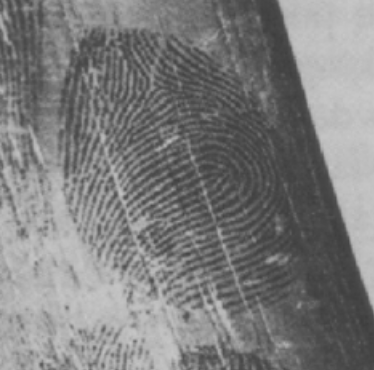
\includegraphics[width=\linewidth]{obrazky-figures/latentny_odtlacok-Drahansky.png}
      \caption{latentný}
      \label{obr:latentny_odtlacok}
    \end{subfigure}
    \caption{Rôzne typy odtlačkov prsta. Obrázky prevzaté z \cite{Drahansky}.}
    \label{obr:druhy_odtlackov}
  \end{figure*}
  
  Latentný odtlačok prsta (\ref{obr:latentny_odtlacok}) je zastrešujúci pojem pre odtlačky prstov náhodne zanechané na povrchoch objektov, obvykle v spojitosti
  s forenznou analýzou. Pod tento pojem niektorí vyšetrovatelia zaraďujú patentné (viditeľné voľným okom), latentné (neviditeľné voľným okom) a plastické odtlačky
  (zanechané v poddajnom materiáli vytvárajúc trojrozmerný odtlačok). Pri zaznamenávaní takýchto odtlačkov sa využívajú špeciálne metódy pre ich vzorkovanie.
  Pri forenznom spracúvaní latentných odtlačkov sa totiž berie na ohľad mnoho vlastností vzorkovaného odtlačku. Medzi tieto vlastnosti môže patriť aj
  chemické zloženie potu zanechaného na povrchu spolu s odtlačkom. Podsekcia čerpala z \cite{FingerprintSrcBook}.

  Táto sekcia čerpala z \cite{Handbook} ak nie je uvedené inak.

  \section{Klasifikácia odtlačkov prsta}
  Prvú klasifikáciu vzorov tvorených papilárnymi líniami na končekoch prstov je možné nájsť v dizertácii českého profesora Jana Evangelisty Purkyně
  z roku 1823 \cite{FingerprintSrcBook}. Začiatkom 20. storočia Edward Henry vyvinul klasifikačný systém, ktorý bol neskôr použitý ako základ pre systém
  automatizovanej identifikácie odtlačkov prsta (AFIS). Tento systém bol vyvinutý FBI pre extrakciu markantov odtlačkov prstov automatizovanými metódami
  za pomoci počítačov.

  Odtlačky prstov je možné skúmať na rôznych úrovniach detailu. Vlastne sa jedná o mieru špecifickosti, podľa akej zaraďujeme vlastnosti
  papilárnych línií na jednotlivých odtlačkoch prstov.

  \textbf{Na prvej úrovni}, najglobálnejšej, sa jedná o takzvané singularity, ktoré sa prejavujú ako náhle zmeny v priebehu papilárnych línií. Tieto 
  zmeny môžu byť časté zakončenia alebo rozdvojenia línií na malej ploche, ktoré tvoria \emph{delty} alebo ostré záhyby v líniách, 
  ktoré tvoria \emph{špirály} a \emph{slučky} definujúce \emph{jadrá} odtlačkov prstov. V praxi sa špirály bežne vynechávajú, pretože ich je možné popísať
  ako dve slučky obrátené proti sebe \cite{Handbook}. V niektorých prípadoch \cite{Drahansky, FingerprintSrcBook} sa dokonca singularity tvorené slučkami
  a špirálami zovšeobecnia iba na jadrá, pričom slučky a špirály sa rezervujú ako názvy tried odtlačkov prstov. Jadro bolo pôvodne definované Henrym \cite{Henry}
  ako \uv{najsevernejší bod najvnútornejšej papilárnej línie.}

  Obecne je na najvyššej úrovni možné každý odtlačok prsta zaradiť do tried na základe informácií o singularitách. Najrozšírenejšie triedenie odtlačkov
  prstov je triedenie podľa Henryho, ktorý definoval šesť hlavných tried podľa tvoreného obrazca papilárnymi líniami. Tieto triedy sú znázornené
  na obrázku \ref{obr:triedy_odtlackov}.

  \begin{figure*}[h]\centering
    \centering
    \begin{subfigure}[b]{0.32\linewidth}
      
\includegraphics[width=\linewidth]{obrazky-figures/placeholder.pdf}
      \caption{oblúk}
      \label{obr:triedy_odtlackov/obluk}
    \end{subfigure}
    \hfill
    \begin{subfigure}[b]{0.32\linewidth}
      
\includegraphics[width=\linewidth]{obrazky-figures/placeholder.pdf}
      \caption{špirála}
      \label{obr:triedy_odtlackov/spirala}
    \end{subfigure}
    \hfill
    \begin{subfigure}[b]{0.32\linewidth}
      
\includegraphics[width=\linewidth]{obrazky-figures/placeholder.pdf}
      \caption{ľavá slučka}
      \label{obr:triedy_odtlackov/lava_slucka}
    \end{subfigure}
    \hfill
    \begin{subfigure}[b]{0.32\linewidth}
      
\includegraphics[width=\linewidth]{obrazky-figures/placeholder.pdf}
      \caption{pravá slučka}
      \label{obr:triedy_odtlackov/prava_slucka}
    \end{subfigure}
    \hfill
    \begin{subfigure}[b]{0.32\linewidth}
      
\includegraphics[width=\linewidth]{obrazky-figures/placeholder.pdf}
      \caption{klenutý oblúk}
      \label{obr:triedy_odtlackov/klenuty_obluk}
    \end{subfigure}
    \hfill
    \begin{subfigure}[b]{0.32\linewidth}
      
\includegraphics[width=\linewidth]{obrazky-figures/placeholder.pdf}
      \caption{dvojitá slučka}
      \label{obr:triedy_odtlackov/dvojita_slucka}
    \end{subfigure}
    \caption{TODO obrazky tried odtlackov podla \cite{Henry}} % TODO: obrazky tried odtlackov podla Henryho
    \label{obr:triedy_odtlackov}
  \end{figure*}

  Klasifikačný systém AFIS využívaný v FBI podľa \cite{FingerprintSrcBook} rozlišuje prvé štyri z tried uvedených v obrázku \ref{obr:triedy_odtlackov}.
  Triedy odtlačkov prsta nie sú v ľudskej populácii distribuované rovnomerne.
  Slučky majú najväčšie zastúpenie a sú pozorovateľné až u 61\% obyvateľstva, špirály u 34\% obyvateľstva a oblúky u zvyšných
  5\% obyvateľstva \cite{sciencing}.

  \textbf{Na druhej úrovni}, taktiež nazývanej lokálna úroveň, pozorujeme markanty. Markanty sú útvary tvorené ukončením alebo
  vetvením papilárnych línií. Tieto útvary je možné detegovať, identifikovať a klasifikovať a následne využiť pri analýze odtlačkov prstov.
  Klasifikácia markantov je obšírnejšia, než triedenie odtlačkov prstov, pričom medzi základné markanty zaraďujeme napríklad
  ukončenie, vidličku, hák, kríženie, bočný kontakt, bod, interval, slučku, most a~priesečnú líniu \cite{Drahansky}. Mnohé z vymenovaných typov majú rôzne
  variácie tvorené reťazením ich základných tvarov ako je možné vidieť na snímkach \ref{obr:markant_vidlicka} a \ref{obr:markant_dvojita_vidlicka}.
  Kvôli veľkému množstvu rôznych typov markantov a zložitosti ich rozlíšeniu automatizovanými systémami sa počet rozpoznávaných markantov v mnohých
  situáciách redukuje, pričom sa často využívajú iba ukončenia a vidličky.

  \begin{figure*}[h]\centering
    \centering
    \begin{subfigure}[b]{0.19\linewidth}
      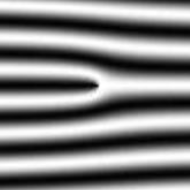
\includegraphics[width=\linewidth]{obrazky-figures/markanty/ukoncenie.png}
      \caption{ukončenie}
      \label{obr:markant_ukoncenie}
    \end{subfigure}
    \hfill
    \begin{subfigure}[b]{0.19\linewidth}
      
\includegraphics[width=\linewidth]{obrazky-figures/markanty/vidlicka.png}
      \caption{vidlička}
      \label{obr:markant_vidlicka}
    \end{subfigure}
    \hfill
    \begin{subfigure}[b]{0.19\linewidth}
      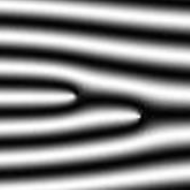
\includegraphics[width=\linewidth]{obrazky-figures/markanty/dvojita_vidlicka.png}
      \caption{dvojitá vidlička}
      \label{obr:markant_dvojita_vidlicka}
    \end{subfigure}
    \hfill
    \begin{subfigure}[b]{0.19\linewidth}
      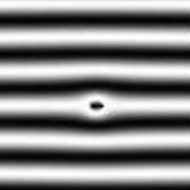
\includegraphics[width=\linewidth]{obrazky-figures/markanty/bod.png}
      \caption{bod}
      \label{obr:markant_bod}
    \end{subfigure}
    \hfill
    \begin{subfigure}[b]{0.19\linewidth}
      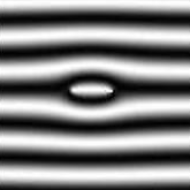
\includegraphics[width=\linewidth]{obrazky-figures/markanty/slucka.png}
      \caption{slučka}
      \label{obr:markant_slucka}
    \end{subfigure}
    \caption{Vybrané typy markantov. Čierne línie reprezentujú vrcholy papilárnych línií. Prevzaté z \cite{Drahansky}.}
    \label{obr:typy_markantov}
  \end{figure*}

  Je vhodné poznamenať, že niektoré páry markantov majú svoje inverzné náprotivky. Túto inverziu je možné vidieť na pároch
  \ref{obr:markant_ukoncenie} a \ref{obr:markant_vidlicka}, prípadne \ref{obr:markant_bod} a \ref{obr:markant_slucka}. Pri oboch pároch je možné invertovať
  hodnoty šedej v snímke a výsledné markanty klasifikovať opačne ako pri originálnych snímkach. Takáto nejednoznačnosť môže spôsobiť problémy pri porovnávaní
  rôznych odtlačkov prstov aj od tej istej osoby, pretože takáto inverzia môže nastať aj pri snímaní odtlačku v dôsledku rôzne aplikovaného tlaku počas
  zaznamenávania odtlačku. Aj z tohto dôvodu sa zaznamenávajú nielen polohy daných markantov, ale aj uhol zvieraný smerom markantu a horizontálnej osi
  snímky, ktorý zostane rovnaký aj pri inverzií z vidličky na ukončenie alebo naopak \cite{Handbook}.

  \textbf{Na tretej úrovni}, najlokálnejšej, sa rozoznávajú detaily kože a atribúty papilárnych línií. Na tejto úrovni je možné pozorovať
  póry, šírku papilárnych línií, jazvy a poranenia kože, kožné ochorenia, atp. Dlhú dobu sa pri automatizovanej analýze detaily na tejto úrovni
  nespracúvali z dôvodu, že pri nižších rozlíšeniach snímok, typicky pod 1000 ppi (bodov na palec - jednotka používaná napr. pri snímačoch a skeneroch),
  tieto detaily nie sú spoľahlivo pozorovateľné \cite{Handbook}. Vylepšovaním snímačov odtlačkov sa však otvorili možnosti detekcie pórov a na ich základe
  zvyšovanie spoľahlivosti porovnávania odtlačkov prstov automatizovanými systémami.

  Jeden z prvých návrhov automatického autentizačného systému pracujúceho s detailmi tretej úrovne uviedli Stosz a Alyea \cite{StoszAlyea}, ktorí predviedli
  uskutočniteľnosť ich návrhu zabezpečením počítača takýmto systémom.
  V roku 2006 Jain, Chen a Demirkus \cite{jain2006pores} predstavili porovnávanie odtlačkov prstov na základe rozšírenia typického porovnávania
  podľa prvých dvoch úrovní detailu o póry z tretej úrovne. Ich metóda spočíva na dvoj-krokovom rozpoznávaní. Najprv podľa detailov druhej úrovne - markantov
  natočia vstupné snímky a následne vygenerujú hodnotenie zhody podľa druhej a tretej úrovne detailu na výreze odtlačku. Úspešnosť detekcie zhody bola touto
  metódou zvýšená. Ich zistenia podporili koncept využívania detailov tretej úrovne pri automatizovanej analýze a to obzvlášť pre odtlačky, resp. časti
  odtlačkov prstov, kde nie je veľké množstvo informácií obsiahnutých na vyšších úrovniach detailu.

  \section{Spracovanie a analýza snímok odtlačkov prstov} \label{sec:analyza}
  %V súčasnosti automatizované analyzátory odtlačkov prstov vyžadujú úpravu zdrojových snímok. Surové snímky odtlačkov totiž nie sú vhodné pre
  %extrakciu informácí pomocou algoritmov. Skôr, než sa zo snímok môžu začať extrahovať vlastnosti ako singularity a markanty je potrebné snímku
  %spracovať tak, aby sa so snímkou pracovalo jednoduchšie pri samotnej analýze.

  %Medzi hlavné kroky spracovania vstupnej snímky patria zníženie šumu snímky, zvýšenie kontrastu a binarizácia snímky a ztenšenie línií.

  Metódy spracovania a analýzy odtlačkov prstov sa líšia na základe požadovanej aplikácie analyzátora. Napríklad pri zabezpečovaní mobilných telefónov
  sa nekladie až taký dôraz na kvalitu analýzy ako napríklad v kriminalistike, a teda sa mnohé časti analýzy preskočia, prípadne
  sa im nevenuje veľká pozornosť za účelom zrýchlenia systému. Avšak hlavná kostra analýzy je vždy relatívne nemenná.

  % //TODO: mozno nejaky obrazok o process flow pri spracovani a analyze pre ilustraciu poradia ukonov

  \subsection{Vylepšenie snímok}
  % //TODO: ak budem moc vyuzivat Hong zdroj, tak napisat sem na zaciatok sekcie, ze je to zalozene na tom zdroji
  Jedným z prvých krokov spracovávania snímok odtlačkov prstov je ich vylepšenie (angl. image enhancement). Väčšina zdrojov odtlačkov je nespoľahlivých
  v zmysle, že nie je možné zaistiť aby boli zdrojové snímky bez signálového alebo iného šumu. To platí hlavne v kriminalistike,
  kde sa často pracuje s latentnými odtlačkami nízkej kvality. Z tohto dôvodu je dôležité vstupnú snímku nejakým spôsobom upraviť tak,
  aby dopad šumu prítomného v snímke a prípadne chýbajúcich alebo narušených častí odtlačku bol minimalizovaný v neskorších krokoch spracovania,
  napríklad pri extrakcii markantov.

  Snímky odtlačkov, prípadne ich oblasti je možné zaradiť do troch kategórii na základe kvality a rozoznateľnosti papilárnych línií:
  \begin{itemize}
    \item \emph{Dobre rozoznateľná oblasť} obsahuje jasne oddelené hrebene od údolí papilárnych línií bez prerušení ich priebehu.
    \item \emph{Poškodená zotaviteľná oblasť} obsahuje malé množstvo narušení priebehu línií ako sú napríklad drobné jazvy, mierne poškodenie
          samotného odtlačku apod., avšak snímka je stále dostatočne jednotná aby z nej bolo možné extrahovať užitočné informácie.
    \item \emph{Poškodená nezotaviteľná oblasť} je oblasť, ktorá je natoľko poškodená, že extrakcia informácií o štruktúrach papilárnych línií
          z nej nemá zmysel \cite{Hong}.
  \end{itemize}
  Operácie vylepšenia snímok majú za úlohu zvýšiť rozoznateľnosť priebehu papilárnych línií v prvých dvoch kategóriách a odstrániť oblasti tretej
  kategórie \cite{Hong}.
  
  Kroky vedúce k vylepšenej snímke však nie sú striktne obmedzené na redukciu šumu. Zvýšenie kontrastu medzi papilárnymi líniami a údoliami medzi nimi
  je taktiež kľúčová k neskorším úpravám snímky.

  \subsubsection{Zvýšenie kontrastu}
  Pre zvýšenie kontrastu snímky je možné využiť vyrovnávanie histogramu. Táto úprava má veľký dopad na zlepšenie kontrastu pri nadmerne tmavých
  alebo nadmerne bledých snímkach. Vyrovnanie intenzít jednotlivých odtieňov šedej má za účinok zvýšenie kontrastu v hmlistej zdrojovej snímke.
  Metódy ekvalizácie histogramu však môžu nežiadúco zvýrazniť šum obsiahnutý v snímke. Z tohto dôvodu sú často využívané modifikované metódy,
  ako napríklad adaptívna ekvalizácia histogramu, v spojení s filtrom.
  
  %//TODO: rozpisat + obrazok
  
  \subsubsection{Gaborova funkcia}
  Gaborova funkcia je využívaná pre zvýšenie kvality snímok znížením šumu v snímke a zachovaním štruktúry papilárnych línií.
  Filter založený na Gaborovej funkcii je však využiteľný nielen pri redukcii šumu obsiahnutého v snímke, ale aj pri zvýšení kontrastu papilárnych línii.
  Jedná sa o orientovateľný sínusový dvojrozmerný filter s pásmovým priepustom, ktorý je schopný tlmiť isté frekvencie, pričom zvýrazňuje iné.
  Tieto vlastnosti sú vysoko žiaduce pri odtlačkoch prstov z viacerých dôvodov. Čiernobiele snímky papilárnych línií sú tvarom sínusové v priebehu
  hodnôt pixelov naprieč líniami v ich normálnom smere a línie sú tiež orientované.
  
  Pretože nie je možné zaručiť, že frekvencia línií je konštantná naprieč celou oblasťou záujmu snímky, snímka sa rozdelí na bloky $h \times w$, 
  pre ktoré je možné diskrétne vypočítať frekvenciu línií a ich orientáciu a teda je možné Gaborov filter vyladiť presne pre jednotlivé bloky.
  

  \subsection{Orientácia}
  Lokálna orientácia papilárnych línií v snímku je uhol zvieraný líniami v jej lokalizovanej časti okolo daného bodu
  s horizontálnou osou snímky. Konkrétnejšie, je to uhol zvieraný líniami v ľubovoľnej oblasti okolo pixelu $[x,y]$ s
  horizontálnou osou snímky. Pri automatizovanej analýze sa často orientácia neprepočítava pre každý pixel z dôvodu zníženia času predspracovania snímky.
  Namiesto toho je možné ju vypočítať diskrétne pre časti snímky a následne interpoláciou takto získaných orientácií je možné aproximovať
  orientáciu papilárnych línií v okolí explicitne vyhodnotenej časti snímky \cite{Handbook}.

  Orientáciu línií je možné vypočítať mnohými spôsobmi, v tejto práci sa však venujem metóde navrhnutej Hongom et al. v \cite{Hong}.
  Táto metóda sa spolieha na výpočet gradientu Sobelovým, prípadne obdobným operátorom. Postup výpočtu je nasledovný:
  \begin{itemize}
    \item Vstupná snímka sa rozdelí na $h \times w$ bloky
    \item Vypočíta sa gradient Sobelovým operátorom
    \item Odhadne sa lokálna orientácia bloku pomocou rovníc:
          \begin{equation}
            \mathcal{V}_x(i,j) = \sum_{u=i-\frac{h}{2}}^{i+\frac{h}{2}}\sum_{v=j-\frac{w}{2}}^{j+\frac{w}{2}} 2\partial _{x}(u,v) \partial _y(u,v),
          \end{equation}
          \begin{equation}
            \mathcal{V}_y(i,j) = \sum_{u=i-\frac{h}{2}}^{i+\frac{h}{2}}\sum_{v=j-\frac{w}{2}}^{j+\frac{w}{2}} (2\partial ^{2}_{x}(u,v) \partial ^{2}_{y}(u,v)),
          \end{equation}
          \begin{equation}
            \theta{}(i,j) = \frac{1}{2}\tan{}^{-1}(\frac{\mathcal{V}_y(i,j)}{\mathcal{V}_x(i,j)}),
          \end{equation}
          kde $\theta{}(i,j)$ je aproximáciou lokálnej orientácie línií metódou najmenších štvorcov pre blok so stredom na pixeli $(i,j)$.
    % //TODO: zvysok bodov zo zdroja Hong, ak treba
  \end{itemize}

  %//TODO: popisat binarizaciu bud v zvlast podsekcii alebo spolu so stenčovaním línií

  \subsection{Frekvencia papilárnych línií}
  Dôležitým krokom, obzvlášť pred následnou úpravou vstupnej snímky frekvenčným filtrom, je výpočet frekvencie papilárnych línií.
  Frekvenciu papilárnych línií v nejakom bode $[x,y]$ je možné definovať ako počet vrcholov pozdĺž výrezu so stredom v danom bode $[x,y]$,
  ktorý je kolmý na lokálnu orientáciu línií $\theta_{xy}$. Frekvencia sa obyčajne počíta pre každý bod snímky odtlačku prsta,
  pretože hustota vrcholov sa môže líšiť aj v rámci jedného prsta \cite{Handbook}.

  Existuje viacero prístupov k odhadnutiu frekvencie vrcholov papilárnych valov. Jednou z nich je metóda navrhnutá Hongom et al. v \cite{Hong},
  ktorá priamo analyzuje odtiene šedej a ich priebeh v originálnej snímke. Táto metóda priamo aplikuje vyššie uvedenú definíciu na snímku nasledovne:

  \begin{enumerate}
    \item Okno veľkosti $l \times{} w$ sa vytvorí okolo pixelu $[x,y]$. Toto okno je natočené kolmo k smeru priebehu papilárnych línií.
    \item Vypočíta sa $x$-signatúra $X$ spriemerovaním hodnôt pixelov pozdĺž stĺpcov $l$ orientovaného okna.
    \item V prípade, že v orientovanom okne sa nenachádzajú markanty alebo singulárne body, je získaná $x$-signatúra formou sínusová. Vďaka tomu je
          možné frekvenciu medzi vrcholmi vypočítať ako inverziu priemerného počtu pixelov medzi jednotlivými vrcholmi papilárnych línií.
  \end{enumerate}
  Papilárne línie však nemajú uniformný priebeh naprieč celým odtlačkom. V takýchto prípadoch, keď sa v orientovanom okne nachádzajú oblasti, ktoré narúšajú
  hladký sínusový priebeh línií, Hong aplikuje interpoláciu frekvencií z okolitých blokov snímky, čím aproximuje frekvenciu pre danú oblasť. Hong taktiež uvádza
  priemernú frekvenciu línií medzi $1/3$ a $1/25$, na základe ktorej prahuje vypočítané frekvencie na platné a neplatné.

  \begin{figure}[h]
    \centering
    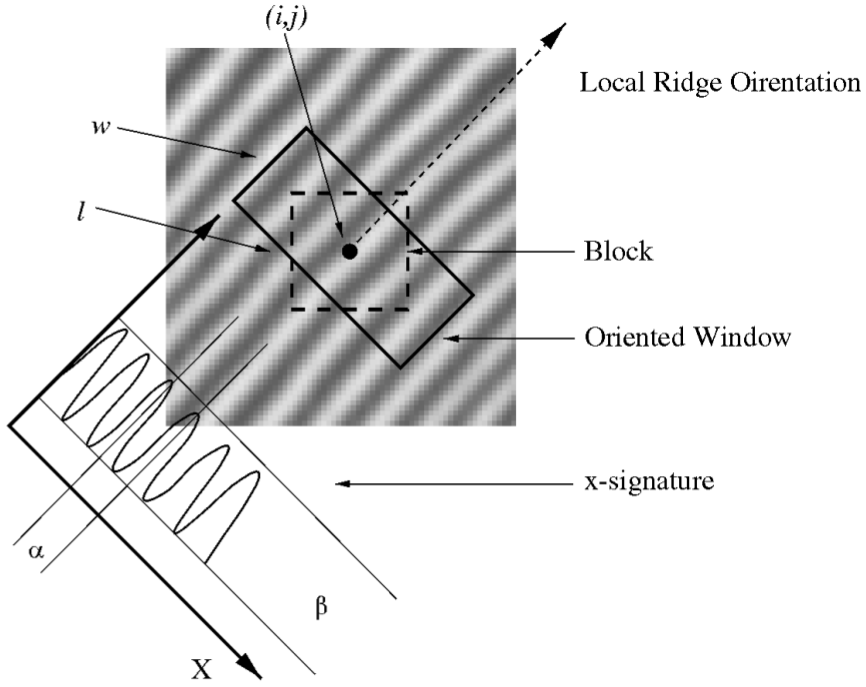
\includegraphics[width=0.8\linewidth]{obrazky-figures/frekvencia-Hong.png} %TODO <- zmenit oznacenia na take ako su v texte tejto subsection
    \caption{Orientované okno naprieč papilárnymi líniami. Prevzaté z \cite{Hong}.}
    \label{obr:frekvencia-Hong}
  \end{figure}

  \section{Spôsoby analýzy markantov}
  Detaily druhej úrovne na odtlačkoch prstov poskytujú veľmi robustné, počítačom analyzovateľné, identifikačné informácie o osobách (v súčasnosti sa vďaka
  zvýšeniu kvality snímok rozširuje automatizovaná analýza aj na tretiu úroveň detailu). Z tohto dôvodu je výskum rôznych metód extrakcie týchto detailov
  obzvlášť rozšírený. Klasifikácia týchto metód je znázornená na diagrame \ref{obr:diagram_extrakcia_markantov}. V tejto sekcii sú popísané niektoré
  z týchto prístupov.

  \begin{figure}[h]
    \centering
    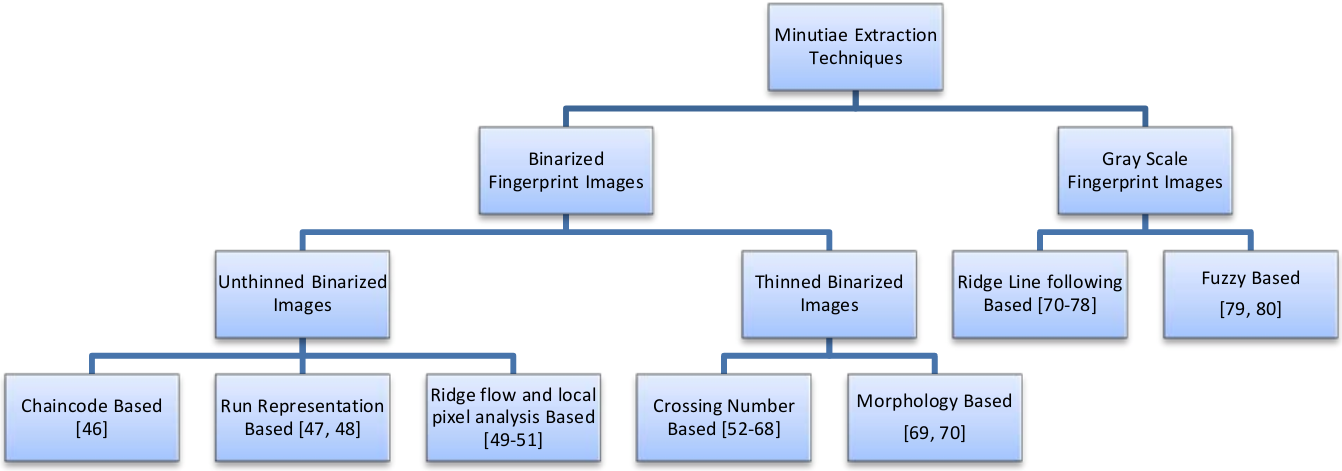
\includegraphics[width=0.8\linewidth]{obrazky-figures/klasifikacia_extrakcie_markantov.png}
    \caption{TODO prerobit tento obrazok z \cite{bansal2011minutiae} na vektorovy (priamo v latexe cez tikz alebo inac).}
    \label{obr:diagram_extrakcia_markantov}
  \end{figure}

  \subsection{Binarizované snímky}
  Snímky odtlačkov prstov, ktoré boli prevedené zo snímok s odtieňmi šedej na snímky binárne, resp. výlučne čierno-biele, fungujú na základe skúmania
  lokalizovaného okolia jednotlivých pixelov. Rozoznávajú najmä vzory tvorené kombináciami pixelov v tomto okolí.

  \subsubsection{Run-length kódovanie}
  Jedná sa o spôsob extrakcie markantov na binarizovaných snímkach odtlačkov prstov bez stenčovania papilárnych línií.
  Metóda spočíva v rozpoznaní horizontálnych a vertikálnych behov čiernej v binárnych snímkach. Tieto snímky sú následne reprezentované kaskádou behov,
  pri ktorých sa skontrolujú susediace behy a charakteristické behy. Behy reprezentujú riadky a stĺpce pixelov, ktoré patria papilárnym líniám. Pri určovaní
  behov sa zaznamená pozícia východiskového pixelu a terminálneho pixelu pre daný beh. Následná analýza kaskády behov dokáže určiť jeden z piatich
  prípadov v závislosti od susedných behov:

  \begin{enumerate}
    \item Ne sú prítomné žiadne behy susediace so súčasným behom.
    \item Sú prítomné dva behy susediace so súčasným behom - jeden beh z každej strany.
    \item Je prítomný jeden beh na jednej zo strán súčasného behu.
    \item Sú prítomné dva behy na jednej zo strán súčasného behu.
    \item Je prítomných viac, než dva behy na jednej zo strán súčasného behu.
  \end{enumerate}
  Prípady tri a štyri sú tzv. charakteristické behy, ktoré preukazujú charakteristiky behov pre ukončenia a vidličky v tomto poradí. Druhý prípad je
  tzv. regulárny beh a reprezentuje beh, ktorý je súčasťou priebehu časti papilárnej línie bez markantu. Rozpoznanie charakteristických behov však
  nemusí znamenať, že zodpovedajú ich charakteristickým markantom, pretože iné typy markantov preukazujú charakteristiky ukončenia (napr. bod má dve ukončenia)
  a vidličky (napr. slučka má dve vidličky). Z tohto dôvodu je potrebná následná validácia nájdených charakteristických behov \cite{bansal2011minutiae}.

  \subsubsection*{Extrakcia na základe počtu prechodov}
  Metóda sa aplikuje na binarizované snímky so stenčenými papilárnymi líniami. Je to často využívaná metóda pre jej jednoduchosť výpočtovú rýchlosť.
  Spočíva v počítaní prechodov medzi pixelmi papilárnej línie a pozadím pre každý pixel prislúchajúci papilárnym líniám. Tieto prechody je možné vypočítať
  pomocou masky veľkosti $3\times{}3$ (\ref{obr:maska_CN}), ktorá je priložená na jednotlivé pixely papilárnych línií. Na ohľad sú brané
  hodnoty na okrajoch masky (bunky $P_1$ až $P_8$). Zvoleným smerom sa následne prechádzajú páry pixelov prekrývaných okrajovými bunkami masky a vypočíta
  sa kumulatívny rozdiel medzi jednotlivými pármi pomocou vzorca \ref{rov:crossing_number}. Výsledné číslo $C_N$ reprezentuje počet prechodov medzi
  pixelmi pozadia a popredia snímky (angl. crossing number alebo condition number). Z tohto počtu je možné vyvodiť, že ak $C_N = 2$, tak sa jedná o ukončenie,
  a ak $C_N = 6$, tak sa identifikovala vidlička. Všetky ostatné hodnoty $C_N$ sú ignorované \cite{amengual1997minutiae_extraction}.

  \begin{figure}[h]
    \centering
      \begin{tabular}{ | l | c | r | }
        \hline
        $P_6$ & $P_5$ & $P_4$ \\ \hline
        $P_7$ & $P$ & $P_3$ \\ \hline
        $P_8$ & $P_1$ & $P_2$ \\
        \hline
      \end{tabular}
    \caption{Maska veľkosti $3\times{}3$ používaná pri výpočte prechodov medzi pixelmi popredia a pozadia pri metóde CN.}
    \label{obr:maska_CN}
  \end{figure}

  \begin{equation}
    C_N = \sum_{i=1}^{8} | P_{i+1} - P_{i} |, \quad\text{kde } P_9 = P_1
    \label{rov:crossing_number}
  \end{equation}

  \subsection{Snímky v odtieňoch šedej}
  Obyčajne výpočtovo náročnejšie techniky na extrakciu markantov sú techniky zamerané na extrakciu bez binarizácie vstupnej snímky. Výhodou analýzy
  takto neupravenej snímky je, že sa do štruktúr papilárnych línií nedostanú falošné prvky. Pri binarizácii sa totiž môžu nechcene odstrániť časti
  papilárnych vzorov alebo dokonca vytvoriť falošné vzory v dôsledku nesprávneho prahovania. Pri stenčovaní sa zas môžu vytvárať falošné vedľajšie výbežky
  z hlavných papilárnych línií. Takáto strata informácií o skutočnom priebehu línií je nežiaduca. Z tohto dôvodu sa skúmali aj možnosti analýzy snímok bez
  takýchto úprav.

  \subsubsection*{Extrakcia markantov sledovaním papilárnych línií}
  Princíp tejto metódy spočíva v sledovaní priebehu papilárnych línií na základe informácií o lokálnej orientácii papilárneho vzoru. Sledovanie sa začne
  zvolením počiatočného bodu $[x_c, y_c]$ a počiatočného smeru $\theta{}_c$. Z tohto bodu sa algoritmus v každom kroku presunie na ďalší bod $[x_t, y_t]$,
  na základe smeru $\theta{}_c$ a veľkosti kroku $\mu$, ktorý udáva počet preskočených pixelov v danom smere. V novom bode sa získajú hodnoty šedej
  naprieč prierezovou sekciou, ktorá je vytvorená kolmo na pôvodný smer $\theta{}_c$ a je dĺžky $2\sigma + 1$. Na základe získaných hodnôt šedej sa
  v rámci sekcie nájde lokálne maximum, pozícia ktorého sa označí ako $[x_n, y_n]$. Tento nový bod sa stáva bodom $[x_c, y_c]$,
  vypočíta sa nový smer $\theta{}_c$ a algoritmus začína novú iteráciu. Algoritmus je znázornený na \ref{obr:sledovanie_linii}.

  \begin{figure}[h]
    \centering
    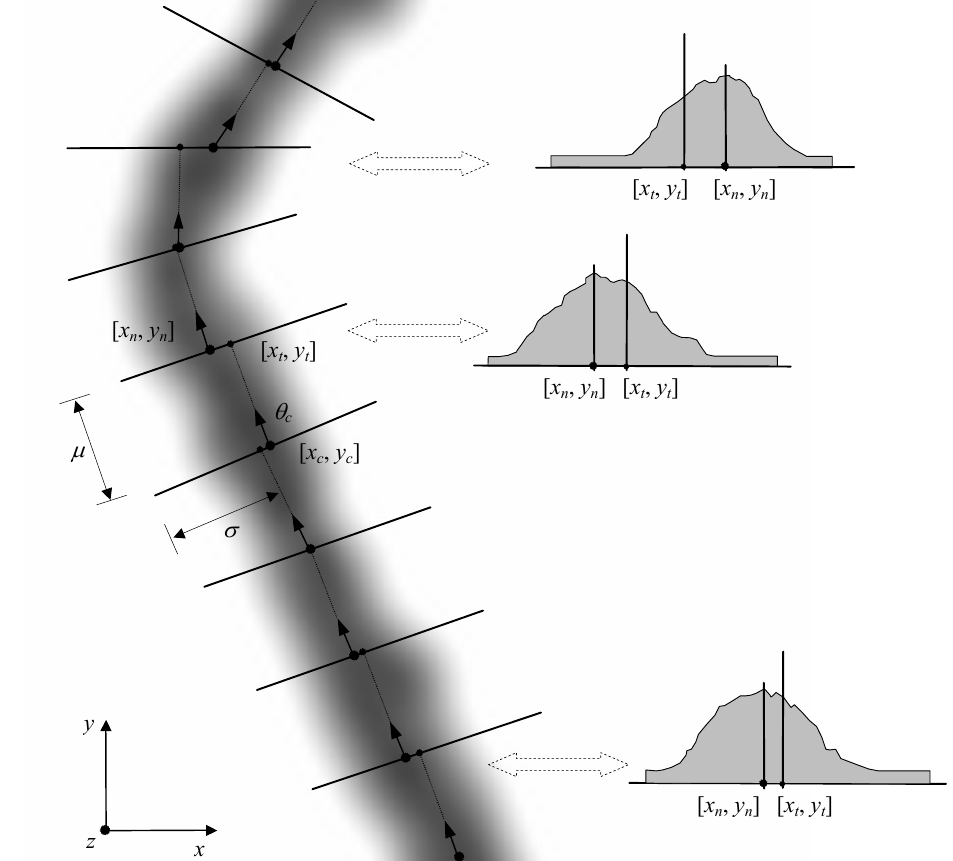
\includegraphics[width=0.65\linewidth]{obrazky-figures/ridge_following-maltoni.png}
    \caption{Znázornenie algoritmu sledovania papilárnych línií. Prevzaté z \cite{Handbook}.}
    \label{obr:sledovanie_linii}
  \end{figure}

  Tento algoritmus je rozširovaný o pomocnú dátovú štruktúru, ktorá zaznamenáva, ktoré časti snímky boli už algoritmom spracované. Toto slúži
  ako prevencia voči viacnásobnému spracovaniu papilárnych línií a zároveň je využívaná pri detekcii markantov. Pomocná snímka $T$ je na začiatku
  extrakcie inicializovaná na prázdnu. Počas sledovania papilárnych línií sa do nej začne ukladať polygonálny obraz skenovaných línií s konštantnou šírkou.
  Na základe porovnávania pomocnej snímky so súčasným krokom sledovacieho algoritmu je možné detegovať pretínanie línií, čo môže znamenať nájdenie markantu
  typu vidlička. Pri ukončených líniách algoritmus deteguje markanty ukončenia \cite{maio1997ridge_following}.

  Existujú variácie vyššie uvedeného algoritmu, ktoré napr. dynamicky upravujú veľkosť kroku $\mu$, alebo ktoré sledujú nielen vrcholy papilárnych línií,
  ale aj susedné údolia \cite{Handbook}.

  \subsection{Stenčovanie línií}
  %//TODO: Stenčovanie línií mozno presunut pod sekciu Spracovanie a analýza snímok odtlačkov prstov
  %LEFT-OFF-HERE
  Tento krok sa vykonáva na binarizovaných snímkach odtlačkov. Jedná sa o stenčenie línií tvorených odtlačkom prsta na čiernobielej snímke na šírku
  jeden pixel. Týmto sa uľahčuje strojová analýza markantov a singularít, pretože po stenčení je možné pracovať iba s \emph{kostrou} odtlačku,
  ktorá obsahuje iba priebeh papilárnych línií vrátane bodov záujmu ako sú spomenuté singularity a markanty, ktoré nezávisia na hrúbke línií.
  
  Samotné stenčovanie však môže do kostry odtlačku zaviesť falošné markanty vďaka nerovnomernosti papilárnych línií v binarizovanej snímke,
  kvôli ktorým sa po ich stenčení vytvoria krátke \uv{chĺpkovité} výbežky z hlavnej štruktúry línií. Existuje mnoho metód navrhnutých na
  zamedzenie vytvárania takýchto falošných výbežkov úpravou binarizovanej snímky, ako napríklad vyplnenie malých dier v líniách, prípadne
  preemptívnou normalizáciou šírky línií pomocou filtra \cite{Handbook}.  

\chapter{Wavelet Scalar Quantization} \label{kap:wsq}
  Koncom dvadsiateho storočia sa veľmi rýchlo rozrastala zbierka snímok odtlačkov prstov v~FBI, pričom tieto snímky pôvodne neboli komprimované,
  čo navyšovalo nároky na úložisko v dátových centrách. Z tohto dôvodu bol vyvinutý algoritmus Wavelet Scalar Quantization (v skratke WSQ).
  Jedná sa o algoritmus vyvinutý na kompresiu snímok odtlačkov prstov, špecificky tých snímaných s rozlíšením 500 ppi. V súčasnosti sa v kriminalistike
  naprieč svetom využívajú snímky v odtieňoch šedej s rozlíšením 500 ppi vo formáte WSQ a 1000 ppi vo formáte JPEG2000 \cite{Libert}.
  Algoritmus WSQ je stratový, čo znamená, že pri kompresii dochádza k istej strate informácií. Pri pomere kompresie 20:1 však spĺňa požiadavky
  pre povolenú stratu informácií z originálnej snímky pre účely kriminalistiky. 
  
  V tejto kapitole sa budem venovať základným prvkom formátu WSQ ako je jeho štruktúra a spôsob kompresie. Informácie boli čerpané zo špecifikácie
  formátu WSQ \cite{WSQSpecification}, ak nie je uvedené inak.

  \section{Štruktúra súboru} \label{sec:struktura}
  % //TODO struktura WSQ (https://web.archive.org/web/20130528173051/http://oreilly.com/www/centers/gff/formats/fbi/index.htm)
  Súbory tvorené snímkami komprimovanými algoritmom WSQ majú definovanú štruktúru. Tieto súbory v sebe nesú informácie potrebné pre úspešnú
  dekompresiu snímok, čo znamená, že obsahujú transformačnú tabuľku, kvantovaciu tabuľku a Huffmanovu tabuľku vrátane ich metadát.
  Samotná štruktúra súboru vo formáte WSQ je podobná tej vo formáte JPEG. Jednotlivé časti súboru sú oddelené dvojbytovými značkami,
  zobrazenými v tabuľke~\ref{tab:znacky_WSQ_suboru}, reprezentujúce začiatky segmentov v súbore. Niektoré segmenty obsahujú dodatočné parametre,
  ktoré popisujú dĺžku, štruktúru a hodnoty daných segmentov.

  \begin{table}
    \caption{Dvojbytové značky vo WSQ súboroch}
    \begin{center}
      \begin{tabular}{ |l c l| }
        \hline
        Značka & Skratka označenia & Vysvetlivka \\
        \hline
        FFA0h       & SOI  & Začiatok snímky \\
        FFA1h       & EOI  & Koniec snímky \\
        FFA2h       & SOF  & Začiatok rámca \\
        FFA3h       & SOB  & Začiatok bloku \\
        FFA4h       & DTT  & Definícia transformačnej tabuľky \\
        FFA5h       & DQT  & Definícia kvantovacej tabuľky \\
        FFA6h       & DHT  & Definícia Huffman tabuľky (tabuliek) \\
        FFA7h       & DRI  & Definícia reštart intervalu \\
        FFA8h       & COM  & Komentár \\
        FFB0h-FFB7h & RSTm & Reštartuj s modulo 8 počet m (kde m=0-7) \\
        \hline
      \end{tabular}
    \end{center}
    \label{tab:znacky_WSQ_suboru}
  \end{table}

  \section{Kompresia}
  Algoritmus kompresie, zobrazený na obrázku \ref{obr:WSQ_diagram}, využíva tri hlavné kroky: diskrétnu vlnkovú transformáciu (DWT) vstupnej snímky
  a jeho kvantovanie a entropické kódovanie kvantovacích indexov.

  \begin{figure}[]
    \centering
    % //TODO prekreslit toto na PDF vektorovy obrazok
    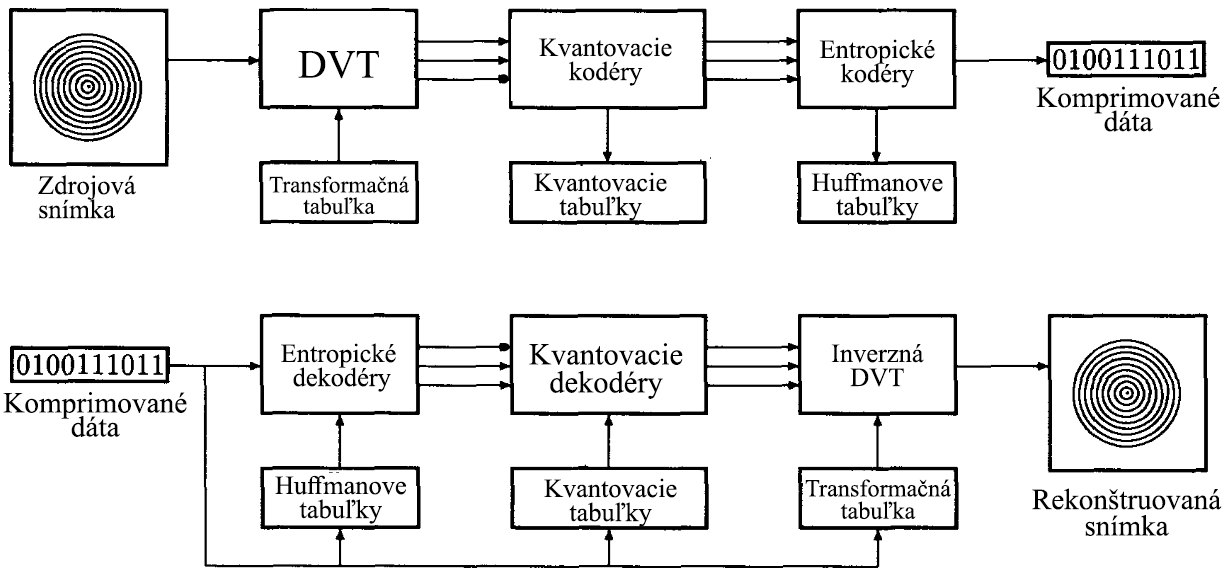
\includegraphics[width=10cm]{obrazky-figures/WSQ_encoder_decoder.png}
    \caption{Diagram WSQ kodéra a dekodéra \cite{Bradley}}
    \label{obr:WSQ_diagram}
  \end{figure}
  
  \subsection{Diskrétna vlnková transformácia}
  Prvým krokom v kompresii snímok vo formáte WSQ je diskrétna vlnková transformácia, ktorá prevedie viacúrovňovú dekompozíciu vstupnej snímky na 
  podpásma. Jedna úroveň transformácie je zobrazená na obrázku \ref{obr:DWT_uroven}. Vstupný signál I je rozdelený na podpásma filtrami horného
  a dolného priepustu, pričom prvý pár filtrov spracúva riadky vstupného signálu a zvyšné dva páry filtrov spracúvajú stĺpce vstupného signálu.
  Kombináciou typu filtrov a smeru filtrovania sa získavajú štyri skupiny koeficientov transformácie v rôznych smeroch: 
  \begin{itemize}
    \item \emph{LL} produkuje aproximáciu vstupného signálu
    \item \emph{HL} produkuje detaily vo vertikálnom smere
    \item \emph{LH} produkuje detaily v horizontálnom smere
    \item \emph{HH} produkuje detaily v diagonálnom smere.
  \end{itemize}
  Po každom filtri sa signál podvzorkuje s faktorom 2, čo znamená, že výsledná veľkosť vektoru jednotlivých koeficientov bude štvornásobne menšia
  z dôvodu podvzorkovania ako riadkov, tak stĺpcov vstupného signálu.

  Jednotlivé podpásma je možné naďalej kaskádovať cez takúto transformačnú banku, kým sa nedosiahne požadovaná úroveň rozkladu vstupného signálu.
  Formát WSQ aplikuje viacúrovňovú dekompozíciu podpásem naznačenú na obrázku \ref{obr:WSQ_DWT_dekompozicia}.
  \begin{figure}[]
    \centering
    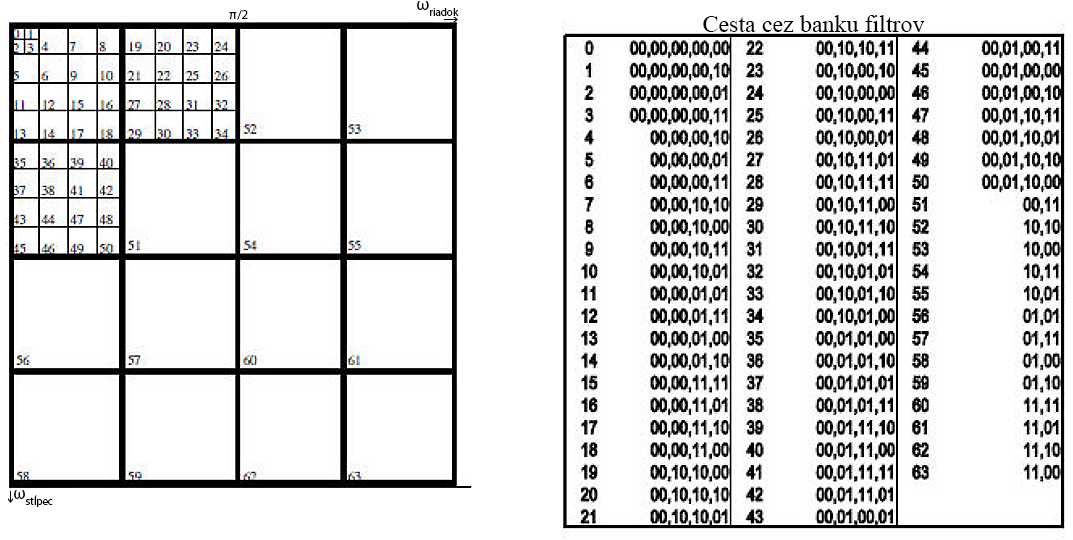
\includegraphics[width=12cm]{obrazky-figures/WSQ_DWT_subband_decomposition.png}
    %//TODO: prekreslit tento obrázok vo vyssej kvalite a podla L/H oznaceni, ktore som vyuzil v tejto sekcii namiesto a_xx ako je vo wsq specifikacii
    \caption{Dekompozícia podpásem vo formáte WSQ.}
    \label{obr:WSQ_DWT_dekompozicia}
  \end{figure}

  \begin{figure}[]
    \centering
    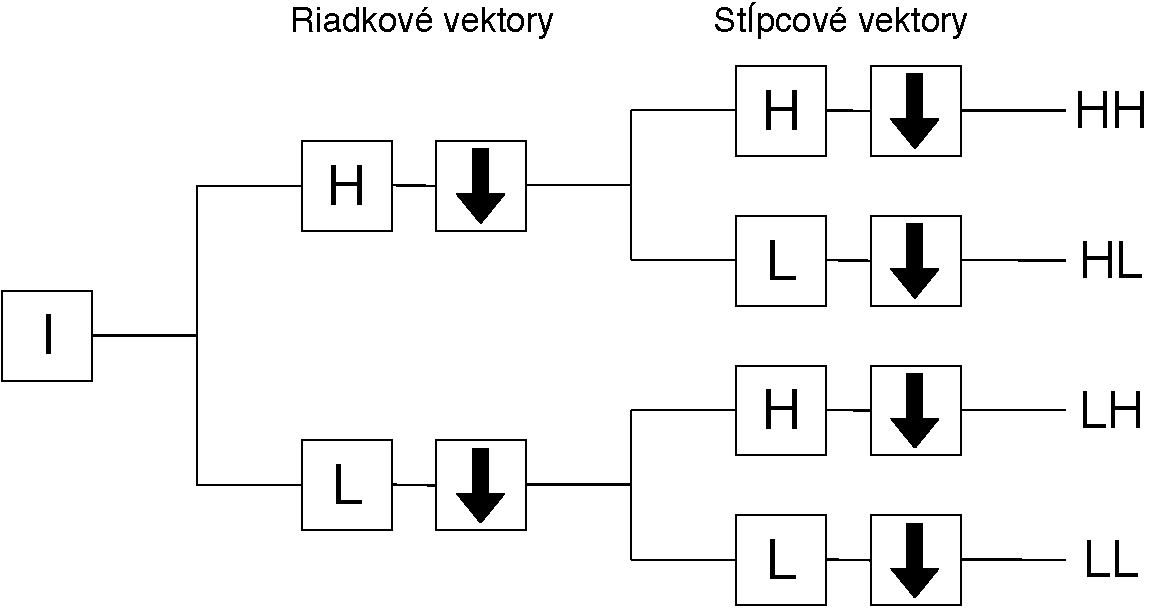
\includegraphics[width=10cm]{obrazky-figures/DWT_level.pdf}
    \caption{Diagram zobrazujúci jednu úroveň rozkladu vstupnej snímky do korešpondujúcich podpásem, kde bloky H predstavujú filtre s horným priepustom,
    bloky L filtre s dolným priepustom, bloky so šípkou nadol značia podvzorkovanie a blok I je vstupný signál.}
    \label{obr:DWT_uroven}
  \end{figure}

  \subsection{Kvantovanie}
  Proces kvantovania je spôsob diskretizácie vstupného signálu. V tomto prípade sa jedná o diskretizáciu koeficientov určených diskrétnou vlnkovou
  transformáciou v predošlom kroku. Jednotlivé koeficienty podpásem získaných transformáciou sú uniformne kvantované v rámci každého podpásma.
  Znamená to, že každé podpásmo môže mať vlastné hodnoty kvantovacieho kroku a šírky kvantovacej \uv{nádoby} (kvantovaného rozsahu). 
  % //TODO: "quantization bin" do slovenciny namiesto "kvantovacia nádoba"...

  Kvantovanie a jeho reverzná operácia pre dekódovanie komprimovaných snímok sú dané vzťahmi \ref{rov:kvantovanie} a \ref{rov:kvantovanie_reverz}:
  \begin{equation}
    p_k(m,n) =
    \begin{cases}
      \lfloor \frac{a_k(m,n) - Z_k / 2 }{Q_k} \rfloor + 1, & a_k(m,n) > Z_k/2 \\
      0, & -Z_k/2 \leq a_k(m,n) \leq Z_k/2 \\
      \lceil \frac{a_k(m,n) + Z_k / 2 }{Q_k} \rceil - 1, & a_k(m,n) < -Z_k/2 \\
    \end{cases}
    \label{rov:kvantovanie}
  \end{equation}
  \begin{equation}
    \hat{a}_k(m,n) = 
    \begin{cases}
      (p_k(m,n) - C)Q_k + Z_k/2, & p_k(m,n) > 0 \\
      0, & p_k(m,n) = 0 \\
      (p_k(m,n) + C)Q_k - Z_k/2, & p_k(m,n) < 0\\
    \end{cases}
    \label{rov:kvantovanie_reverz}
  \end{equation}
  kde index $k$ označuje $k$-te podpásmo, $a_k(m,n)$ označuje koeficient v danom podpásme, $Z_k$ je šírkou nulovej kvantovacej nádoby,
  $Q_k$ je šírkou nenulovej kvantovacej nádoby a $C$ je centrom kvantovacích nádob. $C$ je špecifikáciou daný ako $C = 0,44$ pre najnovší kodér,
  pričom $Z_k$ a $Q_k$ sa získa výpočtom rozptylu jednotlivých podpásem.


  \subsection{Entropické kódovanie}
  Ako predpoklad kódovania špecifikácia určuje rozdelenie snímky do minimálne troch blokov, kde prvá hranica je medzi podpásmami 18 a 19 a druhá
  hranica medzi podpásmami 51 a 52. Je to z dôvodu zabezpečenia progresívneho prenosu, čo znamená, že po sebe nasledujúce bloky pridávajú detaily
  snímky. Vďaka charakteristike dekompozície pomocou DWT prevedenej v prvom kroku kompresie je možné preniesť najvyššiu úroveň aproximácie a
  orientovaného detailu snímky, z čoho je možné rekonštruovať aproximačnú snímku nižšej úrovne. Rozdelením podpásem do blokov na týchto konkrétnych
  indexoch zabezpečí možnosť graduálnej rekonštrukcie snímky pridávaním detailov nižšej úrovne dekompozície,
  ako je zrejmé zo snímky \ref{obr:WSQ_DWT_dekompozicia}. Rozdelenie do viacerých, než troch blokov je vo WSQ tiež možné.

  Pre bezstratovú kompresiu kvantovaných dát sa používa Huffmanovo kódovanie, ktoré využíva početnosť jednotlivých symbolov v datasete pre 
  generovanie čo najkratších kódových slov pre najpočetnejšie symboly. V prípade WSQ sú symbolmi kvantované koeficienty a nulové reťazce
  rôznych dĺžok. WSQ definuje aj špeciálne symboly pre koeficienty a nulové reťazce, ktoré presahujú rozsah kódovacej tabuľky a tieto sú označované
  riadiacou sekvenciou (angl. escape sequence).

\chapter{Návrh aplikácie} \label{kap:navrh_appky}
  \section{Požiadavky}
  Medzi základné požiadavky pre zobrazovač a editor snímok odtlačkov prstov patria podpora štandardných formátov využívaných
  pre ukladanie snímok odtlačkov prstov (napr. WSQ, PNG, BMP),
  detekcia singularít, markantov a triedy odtlačku, ukážka filtrov využívaných pri predspracovávaní odtlačkov prstov.

  Vzhľadom na účel aplikácie, a to demonštrácia spracovania odtlačkov prstov, je vhodné ju navrhnúť tak, aby bola prenositeľná a mala prehľadné 
  grafické rozhranie pre jednoduché využitie študentmi a výskumníkmi nezávisle od ich preferovaného systému.

  \section{Architektúra aplikácie}
  Aplikácia je napísaná v jazyku Python 3.5.3 s využitím väzby na Qt toolkit pre programovanie grafických rozhraní pomocou PyQt.
  % //TODO zistit, ci sa pouzije cx_freeze na freeznutie aplikacie do spustitelneho suboru
  

  \section{Grafické rozhranie}
  Grafické rozhranie pozostáva z ovládacieho panelu, pomocou ktorého je možné vykonávať operácie nad snímkami a z ukážky súčasne
  spracovávaného odtlačku prsta. Ukážka reflektuje úkony vykonávané na snímke pomocou ovládacieho panelu.

  Ovládací panel obsahuje výber jednotlivých filtrov, transformácii a iných úkonov. %//TODO: toto dopisat

  \section{Automatická analýza}
  Režim automatickej analýzy sa drží zaužívaných postupov naznačených v kapitole \ref{kap:odtlacok}. Kroky predspracovania zahŕňajú 
  normalizáciu snímky, filtrovanie Gaborovým filtrom, následnú extrakciu orientácií papilárnych línií, binarizáciu a stenčenie línií.
  
  %Predspracovanie snímky sa začne normalizáciou histogramu

  %\begin{figure}[]
  %  \centering
  %  % //TODO: nakreslit flowchart analýzy
  %  
\includegraphics[width=5cm, height=5cm]{obrazky-figures/placeholder.pdf}
  %  \caption{Kroky automatického analyzátora}
  %  \label{obr:analysis_flowchart}
  %\end{figure}
